\chapter{Einleitung}
\label{cha:Einleitung}

In the rapidly advancing field of cameras and computer vision, the development of robust object recognition models is essential for applications ranging from autonomous systems to surveillance and beyond in many different fields. As technology continues to evolve, the integration of different forms of imaging has become a key focus to enhance the adaptability and reliability of these models. Visible images are affected by environmental and illumination variations such as low lighting and sun glare; meanwhile thermal and infrared images are noisy and have low resolution. \cite[p.1]{SystematicReview23} The main advantage of thermal and infrared imagery is that they are not affected by light conditions, thus they can see objects that would otherwise be very difficult or even impossible to see with visible imagery.

The increasing usage and market size of infrared cameras and imagery (see Figure \ref{fig:marketsize}) and AI-based object detection continuously require better optimized and well performing models, especially in difficult environmental conditions such as rainy, foggy, high and low temperatures. Improvements to these detection methods and systems can have benefits extending into fields such as autonomous vehicles, agriculture, smart cities, search and rescue operations, public safety, security and military. 

\begin{figure}[!ht]
	\centering
		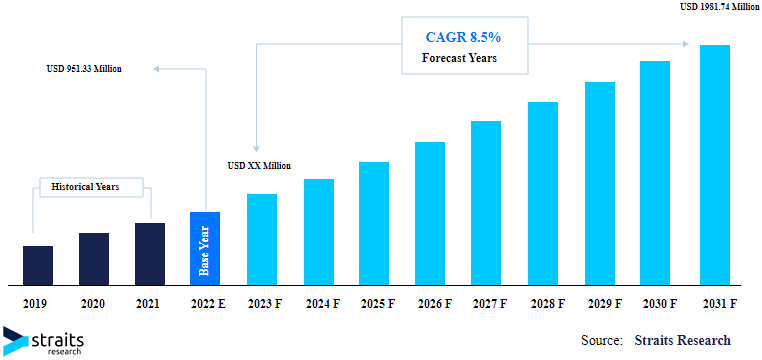
\includegraphics[width=0.75\textwidth]{images/straitsresearch_infrared_camera_marketsize.png}
	\caption{Infrared Camera Market Size \citep{InfraredCameraMarket}}
	\label{fig:marketsize}
\end{figure}

Object detection in the visible spectrum is a field that has seen a lot of interest and progress. Deep learning methods have been developed within the past decade that have continued to bring faster and more accurate detection performances. We could name some of those methods as; R-CNN \citep{girshick2014rcnn}, Faster R-CNN, You Only Look Once(YOLO), Single Shot Detector(SSD)

%TODO: Add references to above methods.


\section{Tabellen}
\label{sec:Tabellen}
Dieser Abschnitt gibt Beispiele für die Verwendung von Tabellen.

\begin{table}[ht]
    \vspace{0.5em}
	\centering
	\begin{tabular}{|l|r|}
        \hline
        Text & 12\% \\
        \hline
        Text & 34\% \\
        \hline
        Text & 56\% \\
        \hline
        Text & 78\% \\
        \hline
        Text & 90\% \\
        \hline
	\end{tabular}
	\caption[Kurztitel Tabelle]{Hier steht der lange Titel für die Tabelle}
	\label{tab:tabelle}
	\vspace{0.5em}
\end{table}

\noindent{}Dies ist lediglich ein Beispiel. Je nach beabsichtigter Aussage, können Tabellen ganz unterschiedlich aussehen. Ein weiteres Beispiel:

\begin{table}[ht]
    \vspace{0.5em}
	\centering
	\begin{tabular}{|c|l|}
		\hline
		\rowcolor[gray]{0.9}\textbf{numbers} & \textbf{text} \\
		\hline
		\hline
		1 & This text flush-left \\
		\hline
		2 & while the numbers are \\
		\hline
		3 & centred \\
		\hline
	\end{tabular}
	\caption[Alternative Tabelle]{Alternative Tabelle mit farbiger Kopfzeile}
	\label{tab:tablealternative}
	\vspace{0.5em}
\end{table}


Das Erstellen von Tabellen kann sehr aufwändig sein. Die folgenden Werkzeuge können hier sehr hilfreich sein:

\begin{itemize}
	\item Excel to \LaTeX{} Converter\\ \url{https://github.com/krlmlr/Excel2LaTeX/releases}
	\item Apple Script: Numbers to \LaTeX{} \\ \url{https://gist.github.com/pgundlach/386384}
	\item Gnumeric (hat eine Export-Funktion für \LaTeX{}): \\ \url{https://projects.gnome.org/gnumeric/}
	\item OpenOffice, Calc2LaTeX: \url{http://extensions.openoffice.org/de/project/calc2latex-macro-converting-openofficeorg-calc-spreadsheets-latex-tables}
\end{itemize}

\section{Tabellen referenzieren}
\label{sec:tabellen_ref}
In diesem Abschnitt werden die Tabellen aus dem vorigen Abschnitt im Text referenziert. Dies ist der Bezug auf die erste Tabelle \ref{tab:tabelle}, und hier der Verweis auf die zweite Tabelle \ref{tab:tablealternative}. Vergeben Sie am besten immer jeder Tabelle, Abbildung, Abschnitt, Kapitel, etc. ein individuelles label, so dass Sie dieses dann zum Referenzieren verwenden können. Im Übrigen stehen Abbildungen und Tabellen niemals für sich alleine, sondern sollten im Text diskutiert werden und somit natürlich auch referenziert. Die Verwendung des "ref{}"-Befehls sorgt dafür, dass immer auf die richtige Nummerierung verwiesen wird, selbst wenn der Text später geändert wird (z.B., wenn Tabellen hinzugefügt oder gelöscht werden). 

\section{Anführungszeichen}
\label{sec:Anfuehrungszeichen}

Es gibt verschiedene Optionen, Anführungszeichen zu generieren. Da das entsprechende Paket eingebunden wurde, können Sie folgende Optionen verwenden:

\begin{itemize}
	\item \enquote{Befehl des Pakets: csquotes}
	\item Alternativ: ``example''
	\item Oder "Beispiel". 
\end{itemize}

Wie Ihnen vielleicht aufgefallen ist, sehen die Alternative etwas anders aus. Für die Verwendung von Anführungszeichen gibt es Konventionen, siehe \url{https://de.wikibooks.org/wiki/LaTeX-W%C3%B6rterbuch:_Anf%C3%BChrungszeichen}





